Implementare un’architettura multi-cloud non significa raggruppare semplicemente vari servizi di diversi Cloud provider in un unico sistema, ma richiede un approccio ragionato ben specifico. L'obiettivo è quello di creare un ambiente coeso che sfrutti in maniera efficace la collaborazione tra i diversi Cloud senza aumentare eccessivamente la complessità necessaria alla sua gestione. A causa della mancanza di standardizzazione, infatti, l'approccio multi-cloud richiede la conoscenza di diversi strumenti in quanto ogni Cloud provider fornisce le proprie API, metodi di accesso e protocolli di sicurezza rendendone difficile l’utilizzo. È facile comprendere come, se da una parte il multi-cloud può portare enormi vantaggi agli utenti che decidono di utilizzarlo, d’altro canto anche le difficoltà da affrontare non sono poche e c'è bisogno di soluzioni efficaci per superarli. \\
La chiave di volta nell’utilizzo del multi-cloud è sicuramente l’astrazione, ovvero l'utilizzo di strumenti che sollevano l'utente dalla necessità di conoscere tutti i dettagli implementativi per la gestione dell'ambiente, permettendo così di ottenere i vantaggi del multi-cloud evitando di introdurre complessità aggiuntiva \cite{ForbesMultiCloud}. Per venire incontro a questa esigenza nasce \textbf{Fly}, un \textbf{Domain-Specific Language} per il Calcolo Scientifico sul multi-cloud il cui obiettivo è quello di semplificare lo sviluppo di applicazioni che sfruttino la potenza computazionale offerta da molteplici Cloud provider, mediante il paradigma FaaS per ottenere alta scalabilità e alte prestazioni. Il punto di forza di Fly risiede nella gestione dell'interazione con il Cloud la quale viene completamente astratta all’utente finale che non necessita di conoscere le specifiche API del provider che vuole utilizzare \cite{ISISLab}. \\
L’aspetto innovativo di Fly è costituito dal concetto di \textbf{funzione Fly}, un blocco di codice indipendente che può essere eseguito in modo concorrente, in linea con il modello FaaS che utilizza funzioni Serverless. \\
Le caratteristiche principali di Fly sono potenza, efficacia ed efficienza:

\begin{itemize}
    \item Fly è \textit{potente} perché permette di sfruttare le capacità di computazione di diversi Cloud provider in una singola applicazione, utilizzando le soluzioni più efficienti in base alle necessità;

    \item Fly è \textit{efficace} perché è un linguaggio user-friendly, facile da comprendere ed utilizzare, che libera il programmatore dal dover gestire e configurare diversi ambienti di esecuzione;
    
    \item Fly è \textit{efficiente} perché permette di scegliere i servizi migliori sia dal punto di vista delle funzionalità che del costo, inoltre riduce i tempi di sviluppo grazie all'astrazione.
\end{itemize}

In questo capitolo saranno descritti i dettagli del linguaggio Fly, descrivendo gli obiettivi per cui è stato sviluppato, la sua architettura e il suo funzionamento. Viene inoltre introdotto il concetto di Domain-Specific Language e Xtext, il framework utilizzato per lo sviluppo di Fly.

\section{Obiettivi}
Fly nasce con lo scopo di riconciliare il Cloud Computing con l’High Performance Computing, fornendo uno strumento potente, semplice ed efficace per lo sviluppo di applicazioni Serverless di Calcolo Scientifico che sfruttino il sistema multi-cloud per ottenere un'alta scalabilità. \\
I principali obiettivi di Fly sono:

\begin{itemize}
    \item \textit{espressività} - possibilità di scrivere algoritmi con poche istruzioni, in modo chiaro e leggibile, in modo da rendere lo sviluppo di un programma di Calcolo Scientifico su larga scala semplice ed intuitivo anche per sviluppatori non esperti;
    
    \item \textit{alta usabilità} - scrivere un programma Fly deve essere semplice per gli esperti del dominio, l’interazione con l’ambiente Cloud deve essere completamente astratta eliminando la necessità di conoscere le API del Cloud provider;
    
    \item \textit{scalabilità} - sia architetture Symmetric Multiprocessing (SMP), sia architetture costruite su Cloud devono essere in grado di scalare facilmente.
\end{itemize}

Fly è stato progettato per permettere agli sviluppatori di dominio, ovvero esperti di un particolare campo con conoscenze limitate riguardo i complessi sistemi paralleli e distribuiti, di sviluppare le proprie applicazioni sfruttando il parallelismo mediante architetture Serverless. Infatti, la sintassi di Fly è ispirata a linguaggi come Java, JavaScript, Python e R, ovvero i più potenti e famosi linguaggi di programmazione utilizzati nel Calcolo Scientifico, in modo da proporre un ambiente familiare agli sviluppatori che lo utilizzano. Vengono forniti numerosi costrutti specifici per il dominio di interesse che vanno a formare un ricco linguaggio utilizzabile facilmente per interagire con i servizi su Cloud. \\
Fly supporta in modo implicito il paradigma di calcolo distribuito e parallelo insieme con la gestione della memoria fornendo inoltre un sistema di comunicazione di processi tramite appositi canali di comunicazione. Un programma Fly è infatti eseguibile sia su un'architettura multiprocessore sia su ambiente Cloud che supporti il modello FaaS, il tutto senza la necessità di conoscere in maniera precisa le risorse di computazione che occorrono per l'esecuzione \cite{ISISLab}.

\section{Domain-Specific Language}
Un \textbf{Domain-Specific Language (DSL)} è un linguaggio di programmazione progettato per essere utilizzato nel contesto di un particolare dominio, fornendo una notazione su misura basata sui concetti e le caratteristiche fondamentali per tale dominio. Un DSL rappresenta il concetto opposto rispetto ai linguaggi General Purpose che invece possono essere usati per un’ampia gamma di problemi e situazioni. Attraverso l’uso di un DSL viene introdotto un livello di astrazione che rende possibile anche ad esperti del dominio la creazione di soluzioni efficaci senza la necessità di avere competenze tecniche specifiche. Questo consente di affidare lo sviluppo di applicazioni software a figure che hanno una conoscenza del contesto più specifica invece che ai soli informatici, permettendo di incrementare l'efficacia e l'efficienza dell'intero processo.\\
Un DSL non ha lo scopo di essere utile a tutti, al contrario è creato per un risolvere problemi relativi ad un contesto molto specifico. Un esempio di linguaggi di questo tipo è HTML progettato per la costruzione di siti web e sicuramente non adatto alla creazione di applicazioni, ad esempio, di simulazione, dominio a cui è invece dedicato OpenABL. Altri DSL noti sono R per l’ambito statistico o SQL per la scrittura di query su database relazionali, il quale offre il vantaggio di non aver bisogno di essere un amministratore di database per scrivere semplici interrogazioni per l'ottenimento di dati. \\
Lo scopo principale di un DSL è quello di essere semplice da imparare e da utilizzare grazie proprio alla specificità di utilizzo che gli permette di essere piccolo, espressivo e poco ridondante, divenendo un punto d’incontro tra esperti del dominio e sviluppatori. \\
La realizzazione di un DSL passa per lo sviluppo di un compilatore che sia in grado di leggere il programma scritto in quel particolare linguaggio, analizzarlo, processarlo e interpretarlo per generare il codice eseguibile. Questo processo prevede una serie di fasi che sono descritte di seguito:

\begin{itemize}
    \item \textit{analisi lessicale} - il programma iniziale viene suddiviso in singole unità chiamate \textit{token}, ognuna delle quali corrisponde ad un singolo elemento del linguaggio;
    
    \item \textit{analisi sintattica} - i \textit{token} identificati vengono analizzati per assicurarsi che formino uno statement valido per il linguaggio. È in questa fase che viene prodotto l’Abstract Syntax Tree (ABS), ovvero la rappresentazione della struttura sintattica del programma;
    
    \item \textit{analisi semantica} - comprende la fase di type checking che controlla che gli assegnamenti di valore siano compatibili con il relativo tipo di dati insieme con la fase di tracciamento degli identificatori, del loro tipo e delle espressioni che si assicura anche che i primi siano stati dichiarati prima dell’uso;
    
    \item \textit{generazione del codice} - parte finale che utilizza i risultati delle fasi precedenti per generare il codice macchina o, eventualmente, il programma scritto in un altro linguaggio.
\end{itemize}

\subsubsection{Xtext}
\textbf{Xtext} \cite{Xtext} è un framework open-source per lo sviluppo di linguaggi di programmazione e DSL. Diversamente dai comuni strumenti disponibili, Xtext genera non solo un parser ma anche un class model per l’Abstract Syntax Tree, fornendo anche un IDE, ovvero un ambiente di sviluppo, basato su Eclipse completo di tutte le funzioni e personalizzabile. Lo sviluppo di un linguaggio attraverso Xtext si basa sulla scrittura di una grammatica che lo definisce in tutte le sue parti, essa permette di ottenere un’infrastruttura completa inclusa di parser, linker, typechecker e compilatore insieme con il supporto all’editing per Eclipse. L’utilizzo di un framework come Xtext offre enormi vantaggi agli sviluppatori di DSL ed è per questo motivo che è stato scelto per la creazione del compilatore source-to-source di Fly.

\section{Architettura}
Utilizzare Fly per implementare la propria applicazione permette all'utente di non preoccuparsi della quantità di risorse necessaria all'esecuzione, in quanto esse vengono stabilite in automatico in base ai requisiti di computazione. Sono supportati modelli di esecuzione sia sincroni che asincroni ed è possibile scegliere tra due ambienti di run-time, ovvero la macchina locale o l'infrastruttura Cloud. Quest'ultima viene considerata come un'architettura di calcolo parallelo utilizzabile per l'esecuzione di codice concorrente grazie a costrutti specifici atti a facilitare l'esperienza dell'utente. \\
Fly risulta in un linguaggio staticamente e fortemente tipizzato che sfrutta varie tipologie di inferenza per determinare il tipo delle variabili e delle costanti dichiarate. Un programma scritto in Fly viene tradotto in automatico dal compilatore in codice Java, nello specifico ogni tipo di dato presente all'interno di Fly ha un suo corrispettivo in quest'ultimo linguaggio, così come le varie funzionalità specifiche del dominio vengono realizzate sfruttando l'ampia gamma di metodi offerti dal linguaggio General Purpose. \\
L’elemento fondamentale di Fly è rappresentato dal concetto di \textbf{funzione Fly}, ovvero una porzione di codice indipendente che eseguita in maniera concorrente, similmente a quanto avviene con le funzioni Serverless del modello FaaS. Le funzioni Fly possono essere eseguite in sequenziale o in parallelo, sia su infrastruttura locale multi-processore che su Cloud mediante l'utilizzo di appositi costrutti che ne permette la definizione, l'esecuzione, la sincronizzazione e la gestione della comunicazione. Quest’ultima viene resa disponibile anche tra processi differenti in esecuzione su diversi ambienti attraverso l'uso di appositi canali di comunicazione virtuali i quali rappresentano il metodo principale per lo scambio di dati tra diverse funzioni Fly. \\ 

\begin{figure}[htbp]
 \centering
 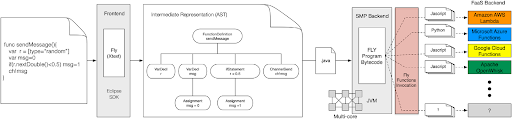
\includegraphics[scale=0.7]{./Figure/FLYCompilazione.png}
 \caption{Flusso di compilazione di Fly.}
 \label{fig:compilazione}
\end{figure}

La \figurename~\ref{fig:compilazione} mostra il \textbf{flusso di una compilazione} in Fly. Partendo da sinistra il programma Fly viene fornito in input al compilatore che genera un \textit{Abstract Syntax Tree (AST)}, ovvero un albero rappresentante la struttura sintattica del codice in cui ogni costrutto corrisponde ad un nodo. Viene definito astratto in quanto non vengono rappresentati tutti i dettagli del codice sorgente ma solo la sua struttura. In seguito la rappresentazione in AST intermedia viene trasformata in un programma Java da cui vengono estratte le singole funzioni Fly, ognuna delle quali verrà tradotta in diversi codici eseguibili, uno per ogni ambiente dichiarato dall’utente. Infine, osservando il lato destro della \figurename~\ref{fig:compilazione} è possibile osservare l’output finale che consiste nel codice compilato delle funzioni Fly pronto per essere eseguito sui vari ambienti dichiarati.

\begin{figure}[htbp]
 \centering
 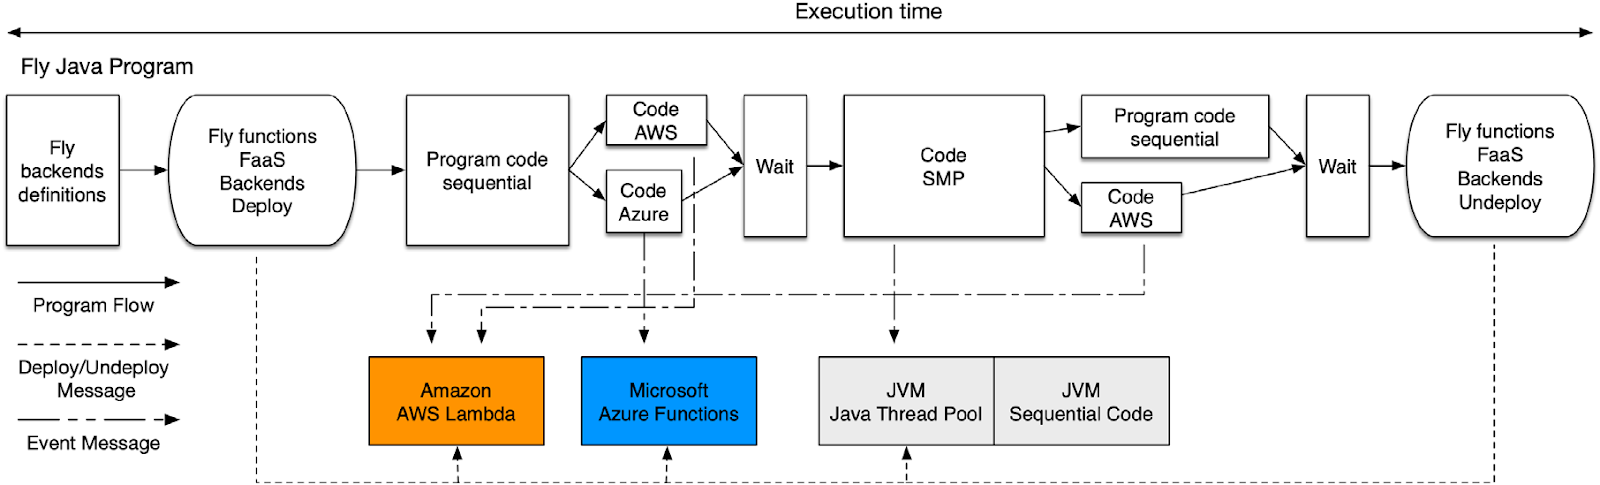
\includegraphics[scale=0.22]{./Figure/FLYEsecuzione.png}
 \caption{Flusso di esecuzione di Fly.}
 \label{fig:esecuzione}
\end{figure}

Nella \figurename~\ref{fig:esecuzione} viene mostrato nel dettaglio il flusso di esecuzione che inizia al lancio di un programma Fly. Seguendo il tempo di esecuzione, la prima fase prevede l’inizializzazione degli ambienti di back-end dichiarati all’interno del codice, questa prevede il login sul Cloud provider e l’istanziazione dei servizi necessari. Il codice generato a partire dalla funzione Fly viene poi caricato sul rispettivo ambiente Cloud, esso risulterà già compilato nel momento in cui il programma principale viene lanciato, in questo modo si evitano i tempi di attesa che sarebbero causati da una compilazione a tempo di esecuzione. Effettuata la fase di inizializzazione il programma principale viene mandato in esecuzione seguendo le istruzioni contenute nel codice Fly e al suo termine vengono effettuate una serie di procedure di undeploy sull’ambiente di back-end, avente lo scopo di eliminare tutte le istanze dei servizi Cloud creati in precedenza.

\section{Definizione del linguaggio}
Fly fornisce diversi tipi di dati che possono essere raggruppati in due insiemi, \textit{basici} e di \textit{dominio}. I primi sono ereditati da Java e comprendono \textit{booleani}, \textit{interi}, \textit{reali} e \textit{stringhe}, essi possono essere usati anche per la dichiarazione di array monodimensionali, bidimensionali e tridimensionali. Di numero maggiore sono invece i tipi di dominio utilizzabili in Fly che permettono all'utente di interagire e comunicare con l'ambiente di esecuzione.\\
Il Listato~\ref{lst:pigreco} mostra un semplice esempio di programma Fly per il calcolo di una stima di Pi Greco tramite il metodo Monte Carlo su ambiente Amazon Web Services, in particolare sfruttando il servizio AWS Lambda \cite{LambdaSite}. È utile fornire una prima descrizione del codice i cui elementi verranno poi approfonditi in seguito. Alla Riga 1 troviamo la dichiarazione dell'ambiente di esecuzione, in questo caso viene definito su AWS. Su tale ambiente è dichiarato un \verb|channel|, Riga 3, che permette al programma principale di comunicare con la funzione Fly \verb|hit| definita alla Riga 5, la quale genera un punto casuale e calcola se appartiene o meno ad un cerchio che abbia origine al punto 1.0, realizzando l'algoritmo per il metodo Monte Carlo. Il valore ottenuto viene poi inviata sul canale \verb|ch|. La funzione \verb|estimation|, Linea 16, legge l'output della funzione \verb|hit| e scrive a schermo la stima di Pi ottenuta. Alla linea 28 è possibile vedere come sono lanciate le funzioni Fly, in particolare viene utilizzata la parola chiave \verb|fly| per eseguire 10000 funzioni \verb|hit| sull'ambiente AWS. Infine l'utilizzo della parola chiave \verb|thenall| fa in modo che quando tutte le funzioni \verb|hit| hanno terminato venga eseguita la funzione \verb|estimation|.\\

\begin{lstlisting}[language=FLY,caption={Stima di PI Greco usando il metodo Monte Carlo su ambiente AWS.}, label={lst:pigreco}]
var local = [type="smp", nthread=4]

var cloud = [type="aws", user="user_name", access_id_key = "access_id_key", secret_access_key="secret_access_key", region="eu-west-2", language="nodejs12.x", thread=2, memory=256, time_=300]

var ch = [type="channel"] on cloud

func hit(){	
    var r = [type="random"]
    var x = r.nextDouble()
    var y = r.nextDouble()
    var msg = 0
    
    if((x * x)+(y * y) < 1.0){msg = 1}
    ch!msg on cloud
}


func estimation(){
    var sum = 0
    var crt = 0
    for i in [0:2] {
        sum += ch? as Integer
        crt += 1
    }
    println "pi estimation: " + (sum*4.0) \ crt
}

fly hit in [0:2] on cloud thenall estimation  
\end{lstlisting}  

\subsubsection{Object} 
Il principale tipo di dato di dominio è il tipo \verb|object|, un insieme eterogeneo di elementi di tipo basico e/o di dominio. Un Fly \verb|object| può essere visto come l'unione di un \verb|array|, un classico vettore, e di una \verb|mappa|, ovvero una struttura dati in grado di memorizzare elementi nella forma di coppie chiave-valore. Il valore di un elemento può essere ottenuto in due diversi modi, utilizzando la sua posizione, come si fa per gli array, o la sua chiave, come nel caso di una mappa. Quando un nuovo valore è assegnato ad una data chiave o posizione viene creato un nuove elemento, altrimenti il nuovo valore va a sostituire il precedente. \\
Ogni tipo di dato di dominio presente in Fly è un'istanza del tipo \verb|object|, questo fa sì che essi siano costruiti tutti con una sintassi simile utilizzando il campo \verb|type| per specificarne il tipo.

\subsubsection{Ambiente di esecuzione}
Il codice di un programma Fly inizia sempre con la dichiarazione di uno o più \textbf{ambienti di esecuzione}, necessari affinché il generatore possa configurare le risorse utili al funzionamento dell'applicazione, in particolare è sempre necessario un ambiente di esecuzione locale corrispondente alla macchina su cui viene lanciato il programma. Ad esempio nel caso di un ambiente locale multiprocessore viene utilizzata una \verb|Java Thread Pool| mentre per gli ambienti su Cloud è necessario creare le istanze dei servizi necessari. Il grande vantaggio offerto da Fly è l'astrazione, dal punto di vista dello sviluppatore infatti tutti i tipi di ambienti possono essere utilizzati allo stesso modo, sarà il compilatore ad occuparsi dei dettagli implementativi specifici relativi al loro utilizzo. \\
La dichiarazione di un ambiente di esecuzione necessita di una serie di parametri che variano in base alla tipologia di ambiente, specificata dal campo \verb|type|. Oltre ad eventuali informazioni aggiuntive richieste dai diversi Cloud provider per accedere ai loro servizi, la dichiarazione relativa ad un'esecuzione su Cloud richiede che l'utente specifichi il linguaggio di programmazione in cui verranno tradotte le funzioni Fly per essere lanciate sul servizio Serverless del provider. In particolare le possibilità sono JavaScript \cite{JavaScriptSite} o Python \cite{PythonSite}.\\
Attualmente gli ambienti supportati sono tre, quattro con l'implementazione trattata in questo lavoro di tesi (vedi Capitolo~\ref{debug}):

\begin{itemize}
    \item \textbf{smp} - ambiente locale che sfrutta il parallelismo basato su un sistema multiprocessore simmetrico sfruttando i thread Java;
    
    \item \textbf{aws} - ambiente su Cloud legato al provider Amazon Web Services (AWS)  \cite{AmazonSite} che sfrutta il servizio AWS Lambda \cite{LambdaSite} per eseguire le funzioni Fly;
    
    \item \textbf{azure} - ambiente su Cloud legato al provider Microsoft Azure \cite{MicrosoftSite} che sfrutta il servizio Azure Function \cite{FunctionSite} per eseguire le funzioni Fly. In questo caso il supporto a Python non è previsto in quanto al momento dell'implementazione non ancora reso disponibile da Azure.
\end{itemize}

\subsubsection{Channel}
La comunicazione e la sincronizzazione sia tra le varie funzioni Fly, sia tra queste e il programma principale avviene mediante la dichiarazione di un \verb|type|\verb|=|\verb|"channel"| che necessita di specificare l'ambiente di esecuzione sul quale funzionare mediante la parola chiave \verb|on|. Questo metodo di comunicazione segue il modello delle code di messaggi bloccanti, ovvero quando si tenta di ricevere un messaggio l'esecuzione si ferma fino a che un nuovo messaggio non viene ricevuto. L'utilizzo del carattere \verb|"!"| permette l'invio di messaggi, vedi Riga 13 del Listato~\ref{lst:pigreco}, mentre il carattere \verb|"?"| è necessario per la loro ricezione, vedi Riga 22 del Listato~\ref{lst:pigreco}. Fly implementa un meccanismo di serializzazione in quando la comunicazione utilizza le infrastrutture di rete per scambiare messaggi con l'ambiente su Cloud.

\subsubsection{Funzione Fly}
Le \textbf{funzioni Fly} sono già state in parte descritte, esse sono frammenti di codice scritto per realizzare una funzionalità specifica indipendente dal programma principale e da altre funzioni ed eseguibile in maniera concorrente. Queste funzioni sono ben diverse da quelle disponibili in altri linguaggi di programmazione e prendono ispirazione da quelle utilizzate nei linguaggi funzionali.\\
La dichiarazione di una funzione Fly è possibile utilizzando la parola chiave \verb|func| a seguito della quale si definisce il nome della funzione e si inseriscono eventuali parametri di input tra parentesi che vengono passati per copia e sono considerati immutabili. Le funzioni Fly possono restituire un valore mediante l'uso della parola chiave \verb|return| ed hanno scoping privato, ovvero solo i parametri della funzione e le variabili locali sono visibili all'interno del corpo della funzione. Per superare tale limitazione possono essere utilizzati sia gli oggetti \verb|channel| che le costanti a patto che la dichiarazione e l'accesso avvengano nello stesso ambiente di esecuzione. Questo significa che se una funzione è in esecuzione sull'ambiente X essa può utilizzare canali e oggetti disponibili su tale ambiente X a prescindere da chi li abbia dichiarati.
Le funzioni Fly possono essere eseguite in modo concorrente utilizzando la parola chiave \verb|fly|, non essendo ammessa la ricorsione essa non può essere utilizzata all'interno del corpo di una funzione. Il suo utilizzo causa la generazione di un evento sull’ambiente che si sta utilizzando, sia esso SMP o su Cloud, in modo che le funzioni vengano eseguite, in linea con il modello di programmazione event-driven che caratterizza il Serverless Computing. Il parallelismo esplicito da cui è caratterizzato Fly è racchiuso nel modo in cui vengono lanciate le funzioni, a seguito della parola chiave \verb|fly| viene dichiarata il nome della funzione da eseguire e, se necessario, il loro numero insieme alla variabile che rappresenta l'ambiente di esecuzione da utilizzare specificato in seguito alla parola chiave \verb|on|.

\subsubsection{Funzione di Callback}
Le \textbf{funzioni di Callback} sono funzioni Fly che vengono eseguite al termine dell'esecuzione di una precedente funzione. Esse possono essere dichiarate dopo la specifica dell'ambiente di esecuzione su cui deve essere eseguita una funzione Fly. Due tipi di funzioni di Callback sono supportate, la prima riguarda quelle specificate in seguito alla parola chiave \verb|then| che indica che la sua esecuzione deve avvenire dopo ogni singola funzione Fly, mentre utilizzando la parola chiave \verb|thenall| si richiede che la funzione venga eseguita solamente quando tutte le funzioni Fly hanno terminato.

\subsubsection{Esecuzioni asincrone}
Fly permette \textbf{esecuzioni asincrone} attraverso l'uso della parola chiave \verb|async| e tipo di dato di dominio chiamato \verb|async-object| che permette all'utente di controllare ed interagire esse. Invocando una funzione utilizzando \verb|async| viene restituito immediatamente il controllo al programma principale in modo che l'esecuzione possa continuare, a questo punto l'utente può controllare lo stato delle funzioni asincrone usando il metodo \verb|status()| dell'\verb|async-object|, mentre il metodo \verb|wait()| mette in pausa l'esecuzione fino a che tutte le funzioni non hanno terminato.

\subsubsection{Codice nativo}
La possibilità di includere \textbf{codice nativo} all'interno di applicazioni Fly è data dalla parola chiave \verb|native|, tale funzionalità consente, ad esempio, di inserire in una funzione Fly codice scritto direttamente in Python ed esso non verrà tradotto o modificato dal compilatore Fly ma copiato così com'è. Tramite la parola chiave \verb|require| è inoltre consentito includere ed installare librerie esterne addizionali nell'ambiente di esecuzione.

\subsection{Struttura di un progetto Fly}
Fly utilizza il gestore di pacchetti \textit{Maven} \cite{MavenSite} per la costruzione e la generazione dei progetti. Maven è uno strumento per la gestione di progetti software e di build automation basato sul concetto di \textbf{Project Object Model (POM)}, un file XML che contiene le dipendenze necessarie al funzionamento dell'applicazione. \\
La creazione di un \textbf{progetto Fly} genera due cartelle principali insieme con un file POM, il tutto racchiuso in un progetto Java Maven che include tutte le dipendenze, il programma principale e il codice delle funzioni, il tutto costruito sulla base del programma Fly da parte del compilatore. Attraverso il comando \verb|mvn package| di Maven tale progetto viene utilizzato per la generazione del file \textit{JAR} eseguibile \cite{ISISLab}.\\
Un progetto Fly è così strutturato:

\begin{itemize}
    \item \textbf{cartella \textit{src}} - cartella in cui è posizionato il file con estensione \textit{.fly} contenente il codice del programma scritto in linguaggio Fly;
    
    \item \textbf{cartella \textit{src-gen}} - cartella contenente i file generati dal compilatore che consistono in un file Java e due file di script. Il file Java ha il compito di orchestrare l'intera esecuzione del programma, ovvero l'intero ciclo di vita comprensivo del lancio dei due file di script. Questi ultimi sono file con estensione \textit{.sh} e contengono distintamente i comandi per il deploy delle funzioni Fly e le procedure per l'undeploy. Il file di deploy si occupa di creare il file necessario alla creazione della funzione Serverless sul servizio FaaS del provider definito, comprensivo di codice, librerie e file di configurazione, mentre il file di undeploy ha il compito di ripulire l'ambiente Cloud dalle risorse create;
    
    \item \textbf{file XML \textit{pom.xml}} - unità fondamentale di Maven per la gestione del progetto, si tratta di un file XML che contiene informazioni e i dettagli di configurazione necessari per effettuare la build, nel caso specifico al suo interno sono presenti le librerie necessarie al programma \cite{MavenPom}.
\end{itemize}

\section{Generazione del codice}
Il punto di forza di Fly è quello di fornire un livello di astrazione tale per cui l'utente non deve conoscere le API di ogni Cloud provider per scrivere un programma che sfrutti al meglio i suoi servizi. Tali API restano comunque essenziali per interagire con essi, infatti è il compilatore di Fly che si occupa di prendere in input il programma per tradurlo in codice effettivamente eseguibile. È quello che avviene nella fase di generazione del codice in cui ogni componente scritta in linguaggio Fly viene trasformata nel linguaggio di destinazione, il quale varia a seconda del contesto, come visto nei paragrafi precedenti. Possiamo quindi affermare che il fulcro del compilatore di Fly è sicuramente la parte di generazione di codice che produce un programma diverso in base all’ambiente di esecuzione dichiarato dall’utente. Nel caso di un ambiente multiprocessore il parallelismo viene implementato attraverso l’uso di una \verb|Java Thread Pool| che permette l'utilizzo di thread ai quali viene assegnata una specifica esecuzione, in particolare essa permette di riutilizzare thread precedentemente creati, eliminando il tempo necessario alla loro creazione. Il programma Fly viene quindi eseguito su una \textit{Java Virtual Machine (JVM)} come un classico programma Java, sulla quale viene eseguito anche l’ambiente SMP, assumendo quindi che siano disponibili almeno due core fisici, uno per l’esecuzione del programma e uno per l’ambiente. L'esecuzione su Cloud prevede invece l'utilizzo delle API fornite dal provider di riferimento che consentono di interagire con i servizi disponibili in base ai quali vengono tradotti i vari costrutti e funzionalità di Fly.\\
Il codice generato per le funzioni Fly varia in base all'ambiente di esecuzione scelto, in particolare il linguaggio di destinazione può essere Java, JavaScript o Python in base a quanto specificato dall'utente. In caso di esecuzione su ambiente SMP locale le funzioni sono tradotte in Java, in quanto eseguite su JVM, diversamente dal Cloud i cui servizi FaaS permettono solitamente l'esecuzione di codice in JavaScript o Python. Oltre al linguaggio utilizzato, l’ambiente di destinazione determina anche il modo in cui viene generato lo script di deploy che costruisce il pacchetto di esecuzione contenente codice sorgente e librerie. \\
Durante la fase di esecuzione l'interazione con il Cloud avviene mediante l'utilizzo degli strumenti di \textbf{Command Line Interface} forniti dai vari provider come la \textit{AWS CLI} \cite{awsCLI} o la \textit{Azure CLI} \cite{azureCLI}, mentre le funzioni vengono invocate con delle chiamate \textit{HTTP POST} asincrone, le quali assicurano la minor latenza permettendo al programma di continuare la sua esecuzione in attesa di risposta da parte del servizio.

\subsubsection{Amazon Web Services}
Amazon Web Services mette a disposizione diverse SDK che permettono di interagire con i suoi servizi praticamente con tutti i principali linguaggi di programmazione \cite{awsSDK}. Il programma principale, essendo scritto in Java fa uso delle \textit{AWS SDK for Java} \cite{AwsJavaSDK} che consentono di accedere a tutti i servizi forniti da AWS mediante delle API dedicate. Gli script di deploy e undeploy invece utilizzano la AWS CLI \cite{awsCLI} per creare le istanze di servizi necessarie al funzionamento del programma e per caricare le funzioni Fly e i relativi pacchetti su AWS Lambda. Queste ultime sfruttano la libreria \textit{boto3} per Python \cite{AwsPySDK} e la libreria \textit{aws-sdk} per JavaScript \cite{AwsJsSDK} per interagire con i servizi di AWS.

\subsubsection{Microsoft Azure}
Le SDK di Microsoft Azure soffrono di alcune problematiche di utilizzo derivanti sia dalla difficile integrazione al di fuori dell’IDE VisualStudio Code, sia dalla mancanza di funzionalità per gran parte dei servizi. Per questo motivo il supporto ad Azure passa per l’utilizzo di un servizio REST API che prescinde dal linguaggio di programmazione in quanto basato su operazioni HTML. Le \textit{Representational State Transfer (REST) API} consistono in endpoint specifici per ogni servizio che supportano un insieme di operazioni HTTP i quali forniscono l’accesso alle principali funzionalità di un servizio come la creazione, l’aggiornamento, la cancellazione o l’ottenimento di informazioni. L’utilizzo delle REST API è regolato dall’utilizzo di un token di autorizzazione ottenibile tramite il servizio Azure Active Directory che ne permette l’acquisizione fornendo i propri dati di accesso, in particolare ID, password e TenantID.
\newpage 
Le sezione seguenti analizzano come il codice scritto in Fly viene tradotto dal compilatore nei vari linguaggi di destinazione per generare i file eseguibili. Tutti i Listati mostrati fanno riferimento al programma  per il calcolo di Pi Greco, proposto nella sua interezza nel Listato~\ref{lst:pigreco}.

\subsection{Ambiente di esecuzione}

\subsubsection{Ambiente locale - SMP}
La dichiarazione di un \textbf{ambiente locale} necessita di due parametri, il primo definisce il tipo di ambiente che sarà di \verb|type|\verb|=|\verb|"smp"|, il secondo specifica il numero di thread che dovranno essere utilizzati.\\

\begin{lstlisting}[language=FLY,caption={Dichiarazione di un ambiente di esecuzione locale.}, label={lst:smp}]
var local = [type = "smp", nthread = 4]
\end{lstlisting}

Il codice Java generato risulta in un oggetto \verb|ExecutorService| che semplifica l'esecuzione asincrona, permettendo di eseguire i task in modo concorrente. Esso fornisce automaticamente un insieme di thread con una serie di metodi che permettono di assegnare loro dei task.\\

\begin{lstlisting}[language=Java,caption={Codice generato per l'ambiente di esecuzione locale.}, label={lst:localJava}]
static ExecutorService __thread_pool_local = Executors.newFixedThreadPool(4);
\end{lstlisting}

\subsubsection{Ambiente su Cloud - Amazon Web Services}
L'utilizzo di un ambiente di esecuzione che utilizzi il \textbf{Cloud AWS} è possibile mediante la dichiarazione di una variabile di \verb|type|\verb|=|\verb|"aws"| la quale necessita di una serie di parametri corrispondenti alle caratteristiche necessarie al lancio delle funzioni Serverless su AWS Lambda \cite{LambdaConfiguration}:

\begin{itemize}
    \item \textbf{dati di accesso dell'account AWS}: in ordine sono necessari \verb|user_name|, \verb| access_id_key|, \verb|secret_access_key|;
    \item \textbf{regione}: id della regione su cui si vogliono lanciare i servizi;
    \item \textbf{linguaggio}: linguaggio di programmazione in cui verranno tradotte ed eseguite le funzioni Lambda. Può essere \verb|nodejs| per JavaScript o \verb|python| per Python;
    \item \textbf{thread}: numero di istanze concorrenti da lanciare per l'esecuzione delle funzioni;
    \item \textbf{memoria}: quantità di memoria disponibile per l'esecuzione di una funzione;
    \item \textbf{time}: tempo limite di esecuzione per ogni funzione.
\end{itemize}



\begin{lstlisting}[language=FLY,caption={Dichiarazione di un ambiente Cloud su AWS.}, label={lst:aws}]
var cloud = [type="aws", user="user_name", access_id_key = "access_id_key", secret_access_key="secret_access_key", region="eu-west-2", language="nodejs12.x", thread=2, memory=256, time_=300]
\end{lstlisting}

Nel Listato~\ref{lst:awsJava} vediamo come vengono istanziati i servizi necessari all'esecuzione di un programma Fly utilizzando le informazioni fornite nella dichiarazione dell'ambiente. Tra i servizi troviamo AWS SQS \cite{SQS} per le code di messaggi, AWS IAM \cite{IAM} per l'autenticazione, AWS S3 \cite{S3} per la memorizzazione di dati e AWS Lambda \cite{LambdaSite} per l'esecuzione di funzioni Serverless.\\

\begin{lstlisting}[language=Java,caption={Codice generato per l'ambiente Cloud su AWS.}, label={lst:awsJava}]
static BasicAWSCredentials cloud = new BasicAWSCredentials("access_id_key", "secret_access_key");
		
static AmazonSQS __sqs_cloud  = AmazonSQSClient.builder()
	.withCredentials(new AWSStaticCredentialsProvider(cloud))
	.withRegion("eu-west-2")
	.build();
		
static AmazonIdentityManagement __iam_cloud = AmazonIdentityManagementClientBuilder.standard()
	.withCredentials(new AWSStaticCredentialsProvider(cloud))
	.withRegion("eu-west-2")
	.build();
			
static AWSLambda __lambda_cloud = AWSLambdaClientBuilder.standard()
	.withCredentials(new AWSStaticCredentialsProvider(cloud))
	.withRegion("eu-west-2")
	.build();
			
static AmazonS3 __s3_cloud = AmazonS3Client.builder()
    .withCredentials(new AWSStaticCredentialsProvider(cloud))
    .withRegion("eu-west-2")
    .build();
\end{lstlisting}

\subsubsection{Ambiente su Cloud - Microsoft Azure}
Utilizzare i servizi a disposizione sul \textbf{Cloud di Microsoft Azure} mediante linguaggi di programmazione risulta complesso e macchinoso a causa delle SDK fornite che, attualmente, presentano molteplici mancanze oltre ad una documentazione particolarmente scarna e spesso non aggiornata. Per tale motivo si è scelto di utilizzare il sistema di REST API attraverso delle chiamate \textit{HTTP}. L'integrazione dei servizi di Microsoft Azure all'interno del codice Java generato dal compilatore Fly è resa possibile grazie alla libreria AzureClient sviluppata presso l'ISISLab \cite{Grieco}, la quale permette di superare il problema della frammentazione delle SDK fornendo un'unica interfaccia che permette un più agevole utilizzo dei servizi. La gestione dei servizi di Azure con JavaScript soffre dei medesimi problemi in termini di SDK ed anche in questo caso è necessario utilizzare delle chiamate \textit{HTTP} per utilizzarli, in particolare vengono utilizzate le librerie \textit{axios} \cite{axios} e \textit{qs} \cite{qs}. In entrambi i casi rimane indispensabile il servizio Azure AD \cite{azureAD} per ottenere il \textit{token} di autorizzazione che permette di effettuare tali chiamate.\\
L'utilizzo di un ambiente di esecuzione che utilizzi il \textbf{Cloud Azure} è possibile mediante la dichiarazione di una variabile di \verb|type|\verb|=|\verb|"azure"| la quale necessita di una serie di parametri corrispondenti alle caratteristiche necessarie al lancio delle funzioni Serverless sul servizio Azure Function \cite{azureFunction}:

\begin{itemize}
    \item \textbf{dati di accesso dell'account Azure}: in ordine sono necessari \verb|client_id|,  \verb|tenant_id|, \verb|secret_key|, \verb|subscription_id|;
    \item \textbf{regione}: id della regione su cui si vogliono lanciare i servizi;
    \item \textbf{linguaggio}: linguaggio di programmazione in cui verranno tradotte ed eseguite le funzioni Lambda. Può essere \verb|nodejs| per JavaScript o \verb|python| per Python;
    \item \textbf{thread}: numero di istanze concorrenti da lanciare per l'esecuzione delle funzioni;
    \item \textbf{time}: tempo limite di esecuzione per ogni funzione.
\end{itemize}



\begin{lstlisting}[language=Java,caption={Dichiarazione di un ambiente Cloud su Azure.}, label={lst:azure}]
var cloud = [type="azure", clientID="client_id", tenantID="tenant_id", secret_key="secret_key", subscriptionID="subscription_id", region="France Central", language="nodejs12.x", threads="2", seconds="300"]
\end{lstlisting}

Il codice generato, visibile nel Listato~\ref{lst:azureJava}, comprende la creazione di una variabile istanza della libreria AzureClient necessaria per avviare tutte le procedure relative ai servizi di Azure. In particolare il metodo \verb|init()| si occupa di istanziare tutti i servizi di base indispensabili per l'esecuzione di qualsiasi programma Fly, sfruttando le informazioni fornite nella dichiarazione dell'ambiente per effettuare l'accesso al Cloud. Il metodo \verb|createFunctionApp(...)| invece è adibito alla creazione dell'istanza del servizio Serverless di Azure che permette l'esecuzione delle funzioni.\\

\begin{lstlisting}[language=Java,caption={Codice generato per l'ambiente Cloud su Azure.}, label={lst:azureJava}]
cloud = new AzureClient("client_id",
    "tenant_id",
    "secret_key",
    "subscription_id",
    __id_execution+"",
    "France Central");
    
cloud.init();

cloud.createFunctionApp("flyappcloud","nodejs12.x");
\end{lstlisting}

\subsection{\textit{Channel}}
La dichiarazione di un \verb|type|\verb|=|\verb|"channel"|, ovvero il mezzo di comunicazione e sincronizzazione utilizzato da Fly, necessita come unica specifica l'ambiente di esecuzione su cui dovrà funzionare, come mostrato nel Listato~\ref{lst:flyChannel}. Questo viene specificato mediante la parola chiave \verb|on| e in base ad esso il compilatore genererà un codice differente, adattandolo in modo che sfrutti i servizi di gestione delle code forniti dall'ambiente specificato. In particolare per AWS si utilizza il servizio AWS Simple Queue Service (SQS) \cite{SQS} mentre per Azure si sfruttano i metodi presenti all'interno della libreria AzureClient.\\
La logica di funzionamento dei prevede che ad uno dei thread dell'ambiente locale venga associato il task di lettura della coda rimanendo costantemente in ascolto e non appena vengono intercettati dei messaggi essi vengono immediatamente scritti sul canale sul quale è possibile leggerli.\\

\begin{lstlisting}[language=Java,caption={Dichiarazione di un \textit{Channel} su Cloud.}, label={lst:flyChannel}]
var ch = [type="channel"] on cloud
\end{lstlisting}

\subsection{Script di deploy e undeploy delle funzioni}
Il funzionamento delle funzioni Serverless su un ambiente Cloud richiede una serie di procedure sia per il deploy che per l'undeploy che vengono eseguite mediante gli strumenti di Command Line Interface forniti dai provider, di conseguenza i comandi cambiano in base al Cloud ma al linguaggio utilizzato. Nonostante ciò queste procedure non sono particolarmente diverse tra loro in quanto tutti necessitano, oltre che del codice della funzione, di una serie di file in formato JSON sia per la specifica del ruolo e delle autorizzazione con le quali la funzione viene eseguita sia per indicare le dipendenze del codice. Fly costruisce l'intero pacchetto per l'esecuzione delle funzioni Serverless prima che queste vengano caricate su Cloud, in particolare questo contiene solo i vari documenti JSON ma anche le librerie necessarie per l'esecuzione che vengono installate mediante il gestore di pacchetti \textit{npm} \cite{npm} per JavaScript e \textit{pip} \cite{pip} per Python.\\
Il codice contenuto all'interno degli script può essere suddiviso in sezioni, ognuna delle quali si occupa di una fase necessaria per il funzionamento del programma, descritte di seguito.

\begin{itemize}
    \item\textbf{Verifica dei parametri e dei requisiti} La prima parte dello script si occupa di verificare che siano presenti i parametri necessari all'interazione con l'ambiente di esecuzione per poi salvarli in apposite variabili. Vengono poi effettuati una serie di controlli per assicurarsi che tutte i pacchetti necessari siano installati sulla macchina, come ad esempio le Command Line Interface.
    \item\textbf{Inizializzazione dei servizi} Attraverso la CLI viene inizializzato l'ambiente del provider di riferimento utilizzando i dati di accesso forniti nella dichiarazione dell'ambiente. In particolare per AWS è necessario creare un'istanza del servizio IAM \cite{IAM} mentre per Azure si effettua semplicemente il login.
    \item\textbf{Creazione del virtual env - Python} In caso il linguaggio scelto per la funzione sia Python è necessario creare un \textit{virtual env}, ossia di un ambiente virtuale isolato che l'interprete di Python utilizza per l'installazione di librerie e script.
    \item\textbf{Creazione del progetto locale} Mediante l'uso dei comandi \textit{bash} lo script crea il progetto Fly occupandosi sia della creazione delle cartelle che dei file. È in questa fase che vengono creati i file JSON necessari per configurare il servizio FaaS, contenenti parametri come il tipo di trigger da utilizzare, nel nostro caso HTTP, i permessi e le autorizzazioni.
    \item\textbf{Codice della funzione Fly Serverless} La funzione Fly viene tradotta nel codice scelto, JavaScript o Python, scritto all'interno di un file che viene inserito all'interno del progetto.
    \item\textbf{Deploy della funzione} Le procedure di deploy della funzione cambiano in base al all'ambiente scelto. AWS richiede che le librerie necessarie all'esecuzione siano già presenti all'interno del pacchetto che verrà caricato su Cloud, per questo motivo lo script utilizza i gestori di pacchetti \textit{npm} o \textit{pip} per la loro installazione per poi creare un file \textit{.zip} contenente l'intero progetto che viene usato per il deploy. A causa dei limiti di dimensione che tale pacchetto deve avere viene fatto un controllo aggiuntivo e in caso di superamento si utilizza il servizio di archiviazione S3 \cite{S3}. Il deploy per Azure risulta invece meno macchinoso in quanto le librerie necessarie vengono specificate all'interno di un file di requisiti che permette di mantenere la dimensione del progetto sempre molto contenuta.
    \item\textbf{Undeploy della funzione} Una volta eseguite le varie funzioni Fly lo script di undeploy si occupa di eliminare tutte le istanze dei servizi creati in modo da lasciare l'ambiente Cloud pulito. Questa fase viene effettuata tramite CLI per AWS mentre per Azure si utilizza la libreria AzureClient, di conseguenza lo script di undeploy contiene solo i comandi per effettuare il logout.
\end{itemize}

\subsection{Sincronizzazione}
L'esecuzione delle funzioni Fly su Cloud necessita di un sistema di sincronizzazione in grado di accertarsi che tutte le funzioni Fly abbiano terminato la loro esecuzione. Questo meccanismo viene implementato attraverso una coda di terminazione sulla quale ogni funzione invia un messaggio una volta completata. Mediante l'uso di un contatore il sistema può notificare che tutte le funzioni sono terminate nel momento in cui sono ricevuti tanti messaggi quante sono le funzioni lanciate. La coda di terminazione viene implementata con la stessa logica vista per i \verb|channel| in maniera totalmente astratta all'utente, essa viene creata, gestita ed eliminata dal programma stesso.